\lecture{7}{16 Oct.}{}

\subsection{Is a Large Clique the Only Obstruction?}

The two bounds just proved are of completely different natures. The first is \emph{local}: if \(\chi(G)\) is large because \(G\) contains a \(K_k\), then there is a small piece of \(G\) one can point at and say \emph{this} is why \(k\) colors are needed. The second is \emph{global}: it compares two parameters of the whole graph and says nothing about where the difficulty sits.

It is natural to hope that the local reason is the only one, i.e.\ that a graph with no small dense substructure can always be colored with few colors. The hope is encouraged by what forbidding short cycles does to a graph locally. If \(G\) has no cycle of length \(3\), then the neighborhood \(N(v)\) of any vertex is independent; if moreover \(G\) has no cycle of length \(4\) or \(5\), then for \(w \in N(v)\) the set \(N(w)\) is again independent and meets \(N(v)\) only in \(w\)'s own edge back to \(v\). Continuing, a ball of radius \(r\) around \(v\) is exactly a tree as soon as \(G\) has no cycle of length \(\le 2r\). Trees are \(2\)-colorable, so from close up such a graph looks like it ought to need two colors.

\begin{center}
    \begin{tikzpicture}[thick, every node/.style={font=\small}]
        \coordinate (v) at (0,0);
        \foreach \i/\a in {1/155, 2/122.5, 3/90, 4/57.5, 5/25}
            \coordinate (u\i) at (\a:1.7);
        \foreach \i in {1,...,5} \draw[blue!60!black] (v) -- (u\i);
        \foreach \i/\a in {1/155, 2/122.5, 3/90, 4/57.5, 5/25}{
            \foreach \d in {-13, 0, 13}{
                \draw[red!80!black, thin] (u\i) -- ({\a+\d}:2.9);
                \fill[red!80!black] ({\a+\d}:2.9) circle (1.7pt);
            }
        }
        \draw[gray, dashed] (u3) to[bend left=25] (u4);
        \foreach \i in {1,2,5} \fill[blue!60!black] (u\i) circle (2.2pt);
        \fill[blue!60!black] (u4) circle (2.2pt);
        \fill[orange!85!black] (u3) circle (2.6pt);
        \node[orange!85!black, anchor=east] at ($(u3)+(-0.12,0.02)$) {$w$};
        \fill (v) circle (2.6pt) node[below=2pt] {$v$};
        \node[gray, anchor=west, align=left, font=\footnotesize] at (3.9,2.3)
            {a dashed edge here would close\\a triangle, so $N(v)$ is independent};
        \draw[gray, thin, ->] (3.85,2.3) -- (1.05,1.95);
        \node[anchor=west, align=left] at (3.9,0.7)
            {with no cycle of length $\le 2r$,\\the ball of radius $r$ around $v$\\is a tree, hence $2$-colorable};
    \end{tikzpicture}
\end{center}

Erd\H{o}s showed that this intuition is entirely wrong, and in the strongest possible sense: one may forbid \emph{all} short cycles and still force arbitrarily many colors. Large chromatic number is a genuinely global phenomenon.

\begin{definition}[Girth]\label{def:girth}
    The \vocab{girth} \(g(G)\) of a graph \(G\) is the length of a shortest cycle in \(G\), with \(g(G) \coloneqq \infty\) if \(G\) is a forest.
\end{definition}

\begin{theorem}[Erd\H{o}s, 1959]\label{thm:erdos-girth}
    For all \(k, \ell \in \mathbb{N}\) there is a graph \(G\) with
    \[
        \chi(G) \ge k
        \qquad\text{and}\qquad
        g(G) \ge \ell.
    \]
\end{theorem}

Since \(g(G) \ge \ell\) forbids every cycle of length \(< \ell\), such a \(G\) contains no \(K_3\) at all, so \(\omega(G) = 2\) and the clique bound is useless. The only tool left is the second bound of \autoref{prop:chromatic-bounds}, and that is exactly what the proof uses: we do not try to exhibit a hard-to-color structure, we only make \(G\) large and its independent sets small.

\begin{intuition}
    To get \(\chi(G) \ge k\) from \(\chi(G) \ge \abs{V(G)}/\alpha(G)\) we need \(\alpha(G)\) to be smaller than \(\abs{V(G)}/k\), i.e.\ the graph must have no large independent set. That pushes us to put in \emph{many} edges. High girth pushes the other way: it forbids edges, or at least forbids them from bunching up. The whole proof is the observation that these two demands can be met at once, because a random graph at the right density has very few short cycles --- few enough to delete by hand.
\end{intuition}

\subsection{The Proof Strategy}

The argument is the method of the present chapter, applied to two kinds of defect simultaneously.

\begin{itemize}
    \item Take a random graph \(G(n,p)\).
    \item Show that it has few short cycles, so that \emph{few} is at most \(\frac{n}{2}\) of them.
    \item Show that it has no independent set of size \(\frac{n}{2k}\), or at worst few such sets.
    \item \textbf{Alteration}: delete one vertex from every short cycle and from every large independent set.
\end{itemize}

What is left is a graph of large girth with small independence number and still at least half of the vertices, and \(\chi \ge \abs{V}/\alpha\) turns that into a large chromatic number.

A remark on the bookkeeping before we start: the two defects are counted by two different random variables \(X\) and \(Y\), but they are repaired by one and the same alteration, so what has to be small is the \emph{sum} \(X + Y\). We will therefore aim at \(\mathbb{E}[X + Y] \le \frac{n}{2}\) and let \autoref{lem:first-moment} produce a single graph in which both counts are simultaneously under control.

\begin{definition}[Binomial random graph]\label{def:gnp}
    For \(n \in \mathbb{N}\) and \(p \in [0,1]\), the \vocab{binomial random graph} \(G(n,p)\) is the random graph on the vertex set \([n]\) in which each of the \(\binom{n}{2}\) pairs is an edge with probability \(p\), independently of all the others.
\end{definition}

\subsection{Counting Short Cycles}

\begin{lemma}\label{lem:few-short-cycles}
    Let \(X\) be the number of cycles of length \(< \ell\) in \(G(n,p)\). If \(np \ge 1\), then
    \[
        \mathbb{E}[X] \le \ell \, (np)^{\ell - 1}.
    \]
\end{lemma}

\begin{proof}
    For \(3 \le s < \ell\) let \(\mathcal{E}_s\) be the set of all \(s\)-cycles on the vertex set \([n]\), let \(X_s \coloneqq \abs{\{C \in \mathcal{E}_s : C \subseteq G(n,p)\}}\) be the number of them present, and for \(C \in \mathcal{E}_s\) put
    \[
        X_C = \begin{cases}
            1, & \text{if all edges of } C \text{ are present}, \\
            0, & \text{otherwise},
        \end{cases}
        \qquad\text{so that}\qquad
        X_s = \sum_{C \in \mathcal{E}_s} X_C .
    \]
    An \(s\)-cycle is determined by an ordering of its \(s\) vertices, up to the \(s\) rotations and the \(2\) reflections that give the same cycle, so
    \[
        \abs{\mathcal{E}_s} = \frac{n (n-1) \cdots (n - s + 1)}{2s} \le \frac{n^{s}}{2s}.
    \]
    A fixed \(C \in \mathcal{E}_s\) has \(s\) edges, each present independently with probability \(p\), so \(\mathbb{P}\bigl( C \subseteq G(n,p) \bigr) = p^{s}\). By \autoref{thm:linearity},
    \[
        \mathbb{E}[X_s] = \sum_{C \in \mathcal{E}_s} \mathbb{P}\bigl( C \subseteq G(n,p) \bigr) \le \frac{n^{s}}{2s} \, p^{s} = \frac{(np)^{s}}{2s}.
    \]
    Summing over \(s\) and using that \(np \ge 1\) makes \((np)^{s}\) largest at \(s = \ell - 1\),
    \[
        \mathbb{E}[X] = \sum_{s=3}^{\ell-1} \mathbb{E}[X_s] \le \sum_{s=3}^{\ell-1} \frac{(np)^{s}}{2s} \le \ell \, (np)^{\ell-1}. \qedhere
    \]
\end{proof}

So \(\mathbb{E}[X] = O\bigl( (np)^{\ell-1} \bigr)\), and for this to be \(o(n)\) --- which is what the alteration can afford --- we need
\[
    (np)^{\ell - 1} \ll n
    \iff p \ll n^{\frac{1}{\ell-1} - 1} = n^{- \frac{\ell-2}{\ell-1}}.
\]
This is an \emph{upper} bound on \(p\): too many edges and the short cycles become too numerous to delete.

\subsection{Counting Large Independent Sets}

\begin{lemma}\label{lem:few-indep-sets}
    Let \(a \coloneqq \bigl\lceil \frac{n}{2k} \bigr\rceil\) and let \(Y\) be the number of independent sets of size \(a\) in \(G(n,p)\). If \(n \ge 4k\), then
    \[
        \mathbb{E}[Y] \le 2^{n} \exp\Bigl( - \frac{p \, n^{2}}{16 k^{2}} \Bigr).
    \]
\end{lemma}

\begin{proof}
    For \(T \subseteq V\) with \(\abs{T} = a\) put
    \[
        Y_T = \begin{cases}
            1, & \text{if } T \text{ is independent}, \\
            0, & \text{if not},
        \end{cases}
        \qquad\text{so that}\qquad
        Y = \sum_{\substack{T \subseteq V \\ \abs{T} = a}} Y_T .
    \]
    The set \(T\) is independent precisely when all \(\binom{a}{2}\) pairs inside it are non-edges, so by \autoref{thm:linearity},
    \[
        \mathbb{E}[Y] = \sum_{T} \mathbb{P}(T \text{ independent}) = \binom{n}{a} (1-p)^{\binom{a}{2}}.
    \]
    Now bound both factors. First \(\binom{n}{a} \le 2^{n}\). Second, \(1 - p \le e^{-p}\), and since \(a \ge \frac{n}{2k} \ge 2\) we have \(\binom{a}{2} = \frac{a(a-1)}{2} \ge \frac{a^{2}}{4} \ge \frac{n^{2}}{16k^{2}}\), whence
    \[
        (1-p)^{\binom{a}{2}} \le e^{- p \binom{a}{2}} \le \exp\Bigl( - \frac{p \, n^{2}}{16 k^{2}} \Bigr). \qedhere
    \]
\end{proof}

For \(\mathbb{E}[Y]\) to be \(o(1)\) we need the exponent to beat \(n \log 2\), i.e.\ \(p n^{2} \gg n\), i.e.\ \(p \gg \frac{1}{n}\). This is a \emph{lower} bound on \(p\): too few edges and the graph has large independent sets.

\begin{intuition}
    The proof works because the two constraints
    \[
        \frac{1}{n} \ll p \ll n^{-\frac{\ell-2}{\ell-1}}
    \]
    are compatible: the right-hand exponent is \(-1 + \frac{1}{\ell-1} > -1\), so the window is a genuine power of \(n\) wide, however large \(\ell\) is. Writing \(p = n^{\theta - 1}\), the window is simply \(0 < \theta < \frac{1}{\ell-1}\).
\end{intuition}
\begin{center}
    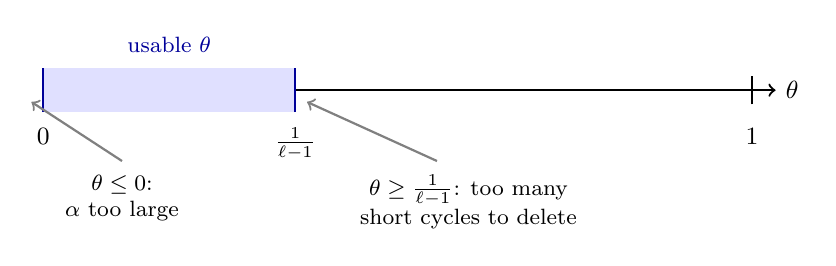
\begin{tikzpicture}[thick, every node/.style={font=\small}]
        \draw[->] (0,0) -- (9.3,0) node[right] {$\theta$};
        \fill[blue!12] (0,-0.28) rectangle (3.2,0.28);
        \draw[blue!60!black] (0,-0.28) -- (0,0.28);
        \draw[blue!60!black] (3.2,-0.28) -- (3.2,0.28);
        \node[anchor=north] at (0,-0.35) {$0$};
        \node[anchor=north] at (3.2,-0.35) {$\frac{1}{\ell-1}$};
        \node[anchor=north] at (9.0,-0.35) {$1$};
        \draw (9.0,-0.18) -- (9.0,0.18);
        \node[blue!60!black, anchor=south, align=center, font=\footnotesize] at (1.6,0.35)
            {usable $\theta$};
        \node[anchor=north, align=center, font=\footnotesize] at (1.0,-0.95)
            {$\theta \le 0$:\\$\alpha$ too large};
        \node[anchor=north, align=center, font=\footnotesize] at (5.4,-0.95)
            {$\theta \ge \frac{1}{\ell-1}$: too many\\short cycles to delete};
        \draw[->, gray] (1.0,-0.9) -- (-0.15,-0.15);
        \draw[->, gray] (5.0,-0.9) -- (3.35,-0.15);
    \end{tikzpicture}
\end{center}

\subsection{Proof of the Theorem}

\begin{proof}[Proof of \autoref{thm:erdos-girth}]
    We may assume \(\ell \ge 4\) and \(k \ge 2\), since otherwise any \(K_k\), resp.\ any graph with a cycle, already works. Fix
    \[
        \theta \coloneqq \frac{1}{2(\ell-1)} \in \Bigl( 0, \tfrac{1}{\ell-1} \Bigr),
        \qquad p \coloneqq n^{\theta - 1},
    \]
    and consider \(G(n,p)\) for \(n\) large. Note \(np = n^{\theta} \ge 1\), so \autoref{lem:few-short-cycles} applies.

    Let \(X\) be the number of cycles of length \(< \ell\), let \(a = \bigl\lceil \frac{n}{2k} \bigr\rceil\) and let \(Y\) be the number of independent sets of size \(a\).

    \emph{Step 1: \(\mathbb{E}[X + Y] \le \frac{n}{2}\).} By \autoref{lem:few-short-cycles},
    \[
        \mathbb{E}[X] \le \ell \, (np)^{\ell-1} = \ell \, n^{\theta(\ell-1)} = \ell \, n^{1/2} = o(n),
    \]
    the point being that \(\theta(\ell-1) = \frac{1}{2} < 1\). By \autoref{lem:few-indep-sets} and \(p n^{2} = n^{1 + \theta}\),
    \[
        \mathbb{E}[Y] \le 2^{n} \exp\Bigl( - \frac{n^{1+\theta}}{16k^{2}} \Bigr)
        = \exp\Bigl( n \log 2 - \frac{n^{1+\theta}}{16k^{2}} \Bigr) = o(1),
    \]
    since \(n^{1+\theta}\) grows faster than \(n\) and \(k\) is a constant. Hence \(\mathbb{E}[X+Y] = o(n) \le \frac{n}{2}\) for \(n\) large enough.

    \emph{Step 2: the alteration.} By \autoref{lem:first-moment} there is a graph \(G_0\) on \([n]\) with \(X + Y \le \frac{n}{2}\): it has at most \(\frac{n}{2}\) short cycles and large independent sets in total. Delete one vertex from each cycle of length \(< \ell\) and one vertex from each independent set of size \(a\), and let \(G\) be the induced subgraph on what remains. Then:
    \begin{itemize}
        \item \(\abs{V(G)} \ge n - (X + Y) \ge \frac{n}{2}\), as we deleted at most one vertex per defect;
        \item \(g(G) \ge \ell\), since every cycle of \(G_0\) of length \(< \ell\) lost a vertex, and passing to an induced subgraph creates no new cycles;
        \item \(\alpha(G) < \frac{n}{2k}\): every \(a\)-set of \(G_0\) that was independent lost a vertex, so no \(a\)-set of \(G\) is independent; as any independent set of size \(\ge a\) contains an independent \(a\)-set, this gives \(\alpha(G) \le a - 1 < \frac{n}{2k}\).
    \end{itemize}

    \emph{Step 3: conclusion.} By \autoref{prop:chromatic-bounds},
    \[
        \chi(G) \ge \frac{\abs{V(G)}}{\alpha(G)} > \frac{n/2}{n/(2k)} = k,
    \]
    and \(g(G) \ge \ell\), which is what we wanted.
\end{proof}

\begin{remark}\hfill
    \begin{enumerate}[(1)]
        \item The case \(\ell = 4\) already says something striking: there are triangle-free graphs of arbitrarily large chromatic number, so \(\chi\) cannot be bounded by any function of \(\omega\).
        \item Nothing in the proof identifies a graph; it is one of the first results for which the probabilistic argument came long before any construction. Explicit constructions of graphs with large girth and large chromatic number do exist --- Lov\'asz gave one in 1968 --- but they are considerably harder than the argument above.
        \item The choice \(\theta = \frac{1}{2(\ell-1)}\) was for definiteness only; any \(\theta \in \bigl( 0, \frac{1}{\ell-1} \bigr)\) works, and pushing \(\theta\) towards the upper end is what the lecture's choice \(p \approx n^{-\frac{\ell-2}{\ell-1}}\) does. Nothing is gained in the statement, since \(k\) and \(\ell\) are fixed constants and \(n\) is free.
        \item The two defects were deleted against a single budget \(\frac{n}{2}\). This is why we needed \(\mathbb{E}[X] = o(n)\) rather than merely \(\mathbb{E}[X] < 1\): the first moment principle is applied once, to \(X + Y\), and produces one graph in which both counts are small at the same time.
    \end{enumerate}
\end{remark}
